\section{Versionsverwaltung}
\subsection{Motivation}
\begin{frame}{Motivation}
	\begin{itemize}
		\item \enquote{Gestern ging es noch \dots}
		\item \enquote{Das Problem hatten wir doch schon Mal \dots}
		\item \enquote{Wer hat den ?\&(\%!\$ verzapft!?}
	\end{itemize}
	\ \\
	\pause
	\ \\
	\begin{block}{Aufgaben}
		\begin{itemize}
			\item Archivierung der Entwicklungsgeschichte
			\begin{itemize}
				\item \enquote{Zeitmaschine}
			\end{itemize}
			\item Koordination paralleler Entwicklungsvorgänge
		\end{itemize}
	\end{block}
\end{frame}

\subsection{Konzepte}
\begin{frame}{Konzepte I}
	\begin{block}{Version/Revision/Commit}
		Eine Momentaufnahme der verwalteten Dateien, verknüpft mit Metadaten wie Autor, Datum und einer Beschreibung
	\end{block}
	\begin{block}{Versionsgeschichte}
		Stellt den Bezug zwischen einzelnen Versionen her
	\end{block}
	\begin{block}{Repository}
		Speichert und verwaltet die Versionsgeschichte sowie die zugehörigen Versionen
	\end{block}
	\begin{block}{Arbeitskopie}
		Ein Abbild einer Version im Dateisystem, an dem auch Änderungen vorgenommen werden können
	\end{block}
\end{frame}
\begin{frame}{Konzepte I}
	\begin{figure}
		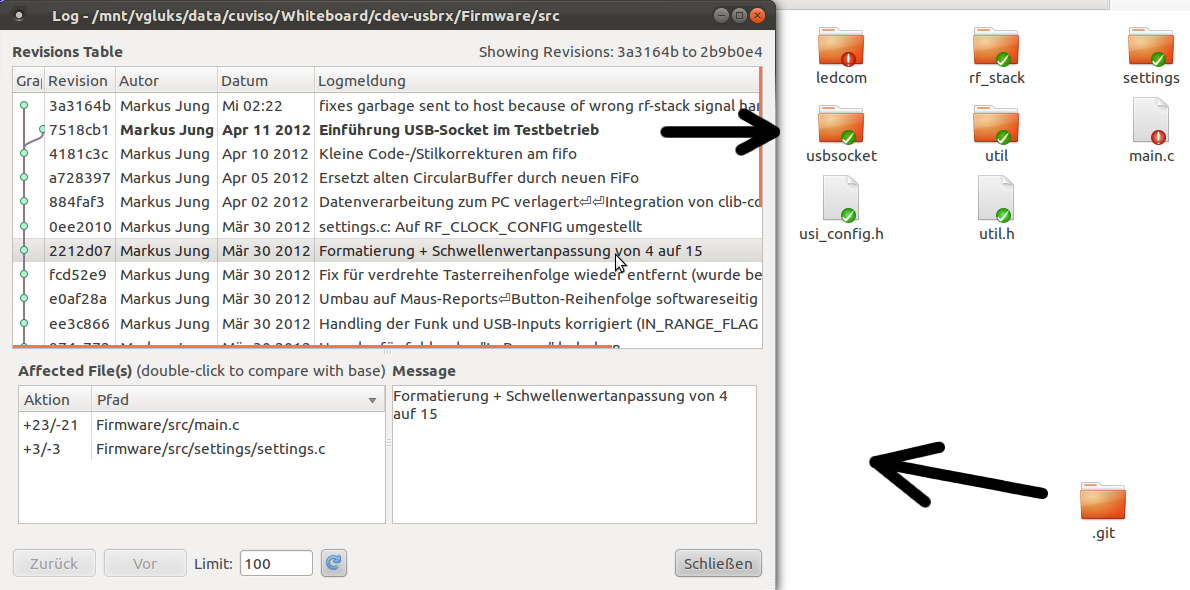
\includegraphics[width=\linewidth]{images/history.png}
	\end{figure}
\end{frame}
\begin{frame}{Konzepte II}
	\begin{columns}
		\column{.1\linewidth}
			\begin{figure}
				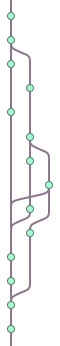
\includegraphics[width=\linewidth]{images/branchmerge.png}
			\end{figure}

		\column{.9\textwidth}
			\begin{block}{Dezentral}
				\begin{itemize}
					\item Jeder Nutzer hat ein (lokales) Repository \\
					\item Erfordert keinen kontinuierlichen Zugriff auf den Server
				\end{itemize}
			\end{block}
			\begin{block}{Branch}
				\begin{itemize}
					\item Softwareentwicklung ist selten linear (\enquote{Entwicklungszweig})
					\item Versionsverwaltungen bilden das durch \enquote{branches} ab
				\end{itemize}
			\end{block}
			\begin{block}{Merge}
				\begin{itemize}
					\item Führt Entwicklungszweige zusammen
					\item Konkurrierende Änderungen können Konfliktlösung erfordern
				\end{itemize}
			\end{block}
			\begin{block}{Tag}
				Markiert Versionen zum schnellen Zugriff
			\end{block}
\end{columns}
\end{frame}

\begin{frame}[fragile]{GIT und github}
	\begin{block}{github}
		\begin{itemize}
			\item Hosting für GIT-Repositories
			\item Für Open-Source-Entwicklung kostenlos
			\item \enquote{social coding}
		\end{itemize}
	\end{block}
	\begin{block}{Fork}
		\begin{itemize}
			\item Eine Abspaltung eines GIT-Repositories
			\begin{itemize}
				\item Jeder \verb|clone| eines Repositories ist eigentlich ein Fork
			\end{itemize}
			\item Eigene Entwicklung finden im eigenen Fork statt
		\end{itemize}
	\end{block}
	\begin{block}{Pull-Request}
		\begin{itemize}
			\item Aufforderung an den Besitzer eines externen Repositories, Änderungen zu übernehmen
		\end{itemize}
	\end{block}
\end{frame}

\subsection{GIT}
\begin{frame}{GIT Workflow}
	\begin{figure}
		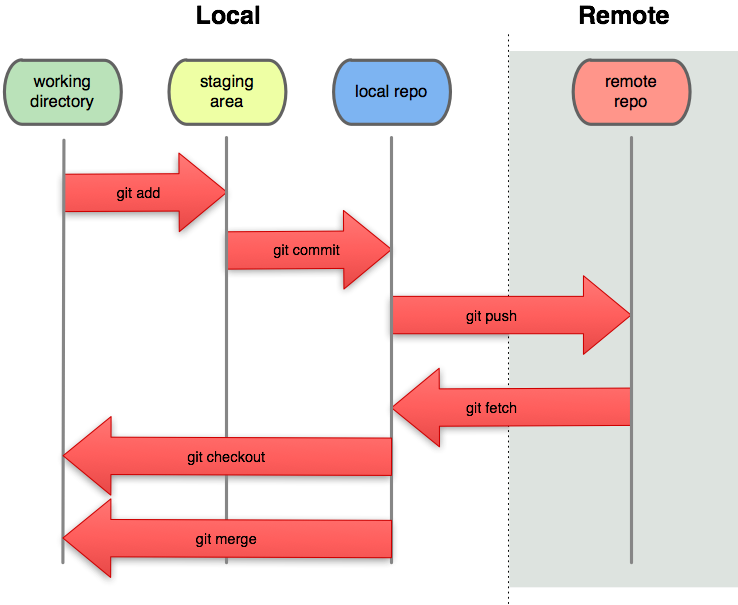
\includegraphics[width=0.75\linewidth]{images/local-remote.png}
	\end{figure}
\end{frame}

\begin{frame}[fragile,allowframebreaks]{GIT Referenz}
	\begin{block}{Repository erzeugen}
		\begin{itemize}
			\item Leeres neues Repository: \verb|git init [<Ordnername>]|
			\item Kopie eines existierenden Repositories: \verb|git clone <URL> [<Ordnername>]|
			\begin{itemize}
				\item Es gibt verschiedene Protokolle zum Zugriff auf ein Repository
				\item SSH ist üblich und bequem, erfordert aber einen SSH-Key
				\item Wir empfehlen daher (bis auf weiteres) die Nutzung von HTTPS
			\end{itemize}
		\end{itemize}
		\begin{figure}
			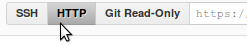
\includegraphics[width=0.5\linewidth]{images/https.png}
		\end{figure}
	\end{block}
	\begin{block}{Änderungen vornehmen}
		\begin{itemize}
			\item Neue/geänderte Datei für die nächste Revision vormerken: \verb|git add <Datei/Ordner>|
			\item Datei aus der Versionskontrolle entfernen: \verb|git rm [--cached] [-r] <Datei/Ordner>|
			\item Vorgemerkte Änderungen verwerfen: \verb|git reset <Datei/Ordner>|
			\item Änderungen übernehmen (neue Revision erzeugen): \verb|git commit [-m "commit message"]| \\
				Commit-Message-Styleguide:
			\begin{itemize}
				\item Eine Zeile Kurzzusammenfassung
				\item Danach ggf. eine Leerzeile und weiterer Text
				\item Zeilenlänge $\le$ 72 Zeichen
			\end{itemize}
		\end{itemize}
	\end{block}
	\begin{block}{Austausch mit anderen Repositories}
		\begin{itemize}
			\item Änderungen an externes Repository übertragen: \verb|git push [--all] [--tags] [<Repository>] [<Branch>]|
			\item Änderungen aus externem Repository beziehen: \verb|git fetch [<Repository>]|
			\item Änderungen aus externem Repository beziehen und anwenden: \verb|git pull [<Repository>]|
			\item Verwaltung externer Repositories: \verb|git remote|
		\end{itemize}
	\end{block}
	\begin{block}{Verzweigungen und ähnlicher Wildwuchs}
		\begin{itemize}
			\item Aktuelle Revision/Branch der Arbeitskopie wechseln: \verb|git checkout [-b] [<Branch>]|
			\item Verwaltung von Branches: \verb|git branch|
			\item Zweig mit eigenem zusammenführen: \verb|git merge <Branch>|
			\item Tagging: \verb|git tag <Tag> [<Revision>]|
		\end{itemize}
	\end{block}
\end{frame}

\subsection{Weiterführende Hinweise}
\begin{frame}[fragile]{Hilfe zur Selbsthilfe}
	\begin{itemize}
		\item \verb|man git| beziehungsweise \verb|git help|
		\item \url{http://help.github.com/} - Github Hilfe
		\item \url{http://www.youtube.com/watch?v=4XpnKHJAok8} \\
			Google Talk "Linus Torvalds on Git"
		\item \url{http://git-scm.com/} - Offizielle Website
	\end{itemize}
\ \\

\tiny
	\begin{itemize}
		\item \url{https://github.com/Gazler/githug} - Interaktives Git Tutorial
		\item \url{http://gitref.org/} - Git Referenz
		\item \url{http://progit.org/book/} - The Pro Git Book
		\item \url{http://gitready.com/} - Git tips and tricks
	\end{itemize}
\end{frame}

